\chapter{Caso d'uso}\label{chp:05-usecase}
%Potremmo dedicare poi un capitoletto con un caso d'uso. Dato il database di moon cloud con questi controlli e queste 
%evaluation si crea la seguente tassonomia. Dato un utente fresh che ha registrato target di 
%questo tipo l'algoritmo ritorna... Dato un altro utente nel db "simile"... così mettiamo tutto insieme.
\begin{figure}[ht!]
    \centering
    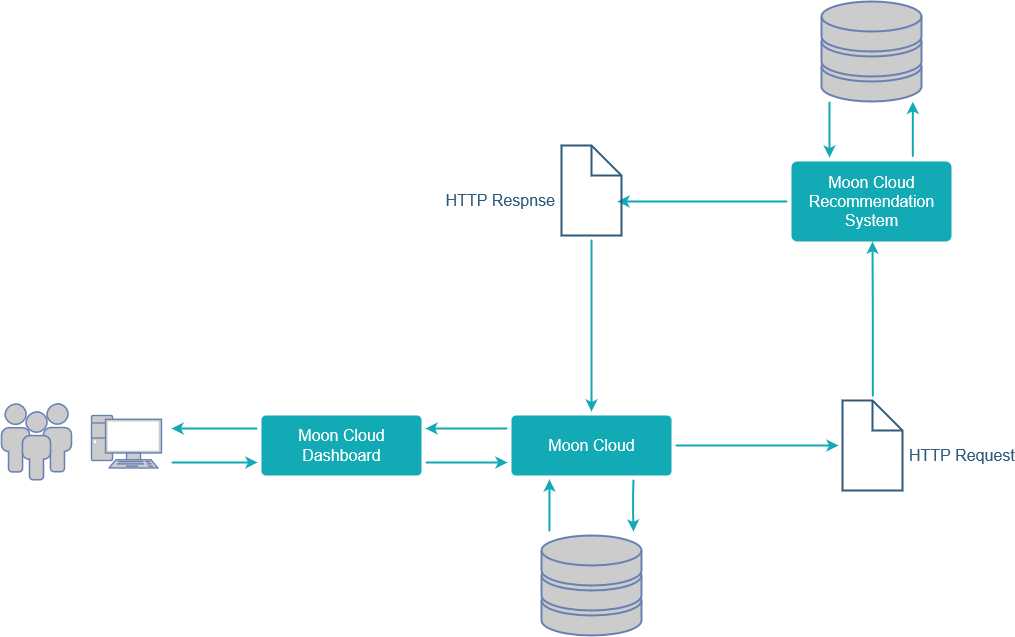
\includegraphics[scale=0.38]{images/UML_MoonCloud_HowToDo.png}
    \caption{.}
    \label{fig:UML_MoonCloud_HowToDo}
\end{figure}
%